\documentclass[11pt,oneside,openany,headings=optiontotoc,11pt,numbers=noenddot]{article}

\usepackage[a4paper]{geometry}
\usepackage[utf8]{inputenc}
\usepackage[T1]{fontenc}
\usepackage{lmodern}
\usepackage[ngerman]{babel}
\usepackage{ngerman}

\usepackage[onehalfspacing]{setspace}

\usepackage{fancyhdr}
\usepackage{fancybox}

\usepackage{rotating}
\usepackage{varwidth}

%Struktogramme
\usepackage[german,curves]{struktex}

\usepackage{pdflscape}
\usepackage{changepage}
\usepackage{graphicx}
\usepackage[bottom]{footmisc}
\usepackage{transparent}
\usepackage{graphbox}
\graphicspath{
	{Pics/PDFs/}
	{Pics/JPGs/}
	{Pics/PNGs/}
}
\usepackage{caption}
\usepackage{wrapfig}
\usepackage{marginnote}
\usepackage{tabularx}
\usepackage{dashrule}
\usepackage{soulutf8}
\usepackage{hhline}
%arydshln suppresses vertical lines in table
%\usepackage{arydshln}
\usepackage{multirow}
\usepackage{enumerate}
\usepackage[hidelinks]{hyperref}
\usepackage{listings}

\usepackage[table]{xcolor}
\usepackage{array}
\usepackage{enumitem,amssymb,amsmath}
\usepackage{interval}
\usepackage{cancel}
\usepackage{stmaryrd}
\usepackage{wasysym}
\usepackage{polynom}
\usepackage{diagbox}
\usepackage{dashrule}
\usepackage{framed}
\usepackage{mdframed}
\usepackage{karnaugh-map}
\usepackage{pdfpages}

\usepackage{blindtext}

\usepackage{eso-pic}

\usepackage{amssymb}
\usepackage{eurosym}

\usepackage[pages=some]{background}
\pagestyle{headings}
\renewcommand{\headrulewidth}{0.2pt}
\renewcommand{\footrulewidth}{0.2pt}
\newcommand*{\underdownarrow}[2]{\ensuremath{\underset{\overset{\Big\downarrow}{#2}}{#1}}}
\setlength{\fboxsep}{5pt}
\newcommand{\explainBelow}[3]{\underbrace{#1}_{\parbox{\widthof{#3}}{\footnotesize\raggedright #2}}}
\newcommand{\explainAbove}[3]{\overbrace{#1}^{\parbox{\widthof{#3}}{\footnotesize\raggedright #2}}}
\newcommand\footnoteref[1]{\protected@xdef\@thefnmark{\ref{#1}}\@footnotemark}


% Codestyle defined
\definecolor{codegreen}{rgb}{0,0.6,0}
\definecolor{codegray}{rgb}{0.5,0.5,0.5}
\definecolor{codepurple}{rgb}{0.58,0,0.82}
\definecolor{backcolour}{rgb}{0.95,0.95,0.92}
\definecolor{deepgreen}{rgb}{0,0.5,0}
\definecolor{darkblue}{rgb}{0,0,0.65}
\definecolor{mauve}{rgb}{0.40, 0.19,0.28}
\colorlet{exceptioncolour}{yellow!50!red}
\colorlet{commandcolour}{blue!60!black}
\colorlet{numpycolour}{blue!60!green}
\colorlet{specmethodcolour}{violet}

%Neue Spaltendefinition
\newcolumntype{L}[1]{>{\raggedright\let\newline\\\arraybackslash\hspace{0pt}}m{#1}}
\newcolumntype{M}{>{\centering\arraybackslash}X}
\newcommand{\cmnt}[1]{\ignorespaces}
%Textausrichtung ändern
\newcommand\tabrotate[1]{\rotatebox{90}{\raggedright#1\hspace{\tabcolsep}}}

%Intervall-Konfig
\intervalconfig {
	soft open fences
}

%Bash
\lstdefinestyle{BashInputStyle}{
	language=bash,
	basicstyle=\small\sffamily,
	backgroundcolor=\color{backcolour},
	columns=fullflexible,
	backgroundcolor=\color{backcolour},
	breaklines=true,
}
%Java
\lstdefinestyle{JavaInputStyle}{
	language=Java,
	backgroundcolor=\color{backcolour},
	aboveskip=1mm,
	belowskip=1mm,
	showstringspaces=false,
	columns=flexible,
	basicstyle={\footnotesize\ttfamily},
	numberstyle={\tiny},
	numbers=none,
	keywordstyle=\color{purple},,
	commentstyle=\color{deepgreen},
	stringstyle=\color{blue},
	emph={out},
	emphstyle=\color{darkblue},
	emph={[2]rand},
	emphstyle=[2]\color{specmethodcolour},
	breaklines=true,
	breakatwhitespace=true,
	tabsize=2,
}
%Python
\lstdefinestyle{PythonInputStyle}{
	language=Python,
	alsoletter={1234567890},
	aboveskip=1ex,
	basicstyle=\footnotesize,
	breaklines=true,
	breakatwhitespace= true,
	backgroundcolor=\color{backcolour},
	commentstyle=\color{red},
	otherkeywords={\ , \}, \{, \&,\|},
	emph={and,break,class,continue,def,yield,del,elif,else,%
		except,exec,finally,for,from,global,if,import,in,%
		lambda,not,or,pass,print,raise,return,try,while,assert},
	emphstyle=\color{exceptioncolour},
	emph={[2]True,False,None,min},
	emphstyle=[2]\color{specmethodcolour},
	emph={[3]object,type,isinstance,copy,deepcopy,zip,enumerate,reversed,list,len,dict,tuple,xrange,append,execfile,real,imag,reduce,str,repr},
	emphstyle=[3]\color{commandcolour},
	emph={[4]ode, fsolve, sqrt, exp, sin, cos, arccos, pi,  array, norm, solve, dot, arange, , isscalar, max, sum, flatten, shape, reshape, find, any, all, abs, plot, linspace, legend, quad, polyval,polyfit, hstack, concatenate,vstack,column_stack,empty,zeros,ones,rand,vander,grid,pcolor,eig,eigs,eigvals,svd,qr,tan,det,logspace,roll,mean,cumsum,cumprod,diff,vectorize,lstsq,cla,eye,xlabel,ylabel,squeeze},
	emphstyle=[4]\color{numpycolour},
	emph={[5]__init__,__add__,__mul__,__div__,__sub__,__call__,__getitem__,__setitem__,__eq__,__ne__,__nonzero__,__rmul__,__radd__,__repr__,__str__,__get__,__truediv__,__pow__,__name__,__future__,__all__},
	emphstyle=[5]\color{specmethodcolour},
	emph={[6]assert,range,yield},
	emphstyle=[6]\color{specmethodcolour}\bfseries,
	emph={[7]Exception,NameError,IndexError,SyntaxError,TypeError,ValueError,OverflowError,ZeroDivisionError,KeyboardInterrupt},
	emphstyle=[7]\color{specmethodcolour}\bfseries,
	emph={[8]taster,send,sendMail,capture,check,noMsg,go,move,switch,humTem,ventilate,buzz},
	emphstyle=[8]\color{blue},
	keywordstyle=\color{blue}\bfseries,
	rulecolor=\color{black!40},
	showstringspaces=false,
	stringstyle=\color{deepgreen}
}

\lstset{literate=%
	{Ö}{{\"O}}1
	{Ä}{{\"A}}1
	{Ü}{{\"U}}1
	{ß}{{\ss}}1
	{ü}{{\"u}}1
	{ä}{{\"a}}1
	{ö}{{\"o}}1
}

% Neue Klassenarbeits-Umgebung
\newenvironment{worksheet}[3]
% Begin-Bereich
{
	\newpage
	\sffamily
	\setcounter{page}{1}
	\ClearShipoutPicture
	\AddToShipoutPicture{
		\put(55,761){{
				\mbox{\parbox{385\unitlength}{\tiny \color{codegray}BBS I Mainz, #1 \newline #2
						\newline #3
					}
				}
			}
		}
		\put(455,761){{
				\mbox{\hspace{0.3cm}
\includegraphics[width=0.2\textwidth]{../../logo.pdf}}
			}
		}
	}
}
% End-Bereich
{
	\clearpage
	\ClearShipoutPicture
}

\setlength{\columnsep}{3em}
\setlength{\columnseprule}{0.5pt}

\geometry{left=1.50cm,right=1.50cm,top=2.50cm,bottom=1.00cm,includeheadfoot}
\pagenumbering{gobble}
\pagestyle{empty}

\begin{document}
	\begin{worksheet}{Berufliches Gymnasium}{Klassenstufe 12 - Informationsverarbeitung}{Lernabschnitt 1: Netzwerke - Adressierung - Subnetting}
		\setcounter{section}{1}
		\setcounter{subsection}{2}
		\subsubsection*{Interessantt IP-Adressen eines Netzes}
		Bevor wir uns mit der Aufteilung eines Netzes in mehrere kleinere Netze befassen, sollte erwähnt werden, dass es in einem Netz immer IP-Adressen mit Sonderrolle gibt (ähnlich zu reservierten Telefonnummern - Polizei 110 oder Feuerwehr).\\
		Die erste Adresse eines Netzes (z.B. 192.168.3.0/24) wie auch die letzte Adresse des Netzes (z.B. 192.168.3.255/24) erfüllen eine besondere Funktion.
		\begin{itemize}[label=-]
			\item Die \textbf{niedrigste}\footnote{Also die erste IP-Adresse eines Netzes, bei der alle Host-Bits auf 0 gesetzt sind.} IP-Adresse eines Netzes haben wir bereits kennengelernt. Sie wird \textbf{Netzadresse} genannt.\\
			Ihre Aufgabe ist die Kennzeichnung des gesamten zugehörigen Netzes von außerhalb.
			\item Die \textbf{höchste}\footnote{Also die letzte I5P-Adresse eines Netzes, bei der alle Host-Bits auf 1 gesetzt sind.} IP-Adresse eines Netzes wird als \textbf{Broadcastadresse} bezeichnet. Sie wird verwendet, wenn innerhalb des Netzes alle Hosts angesprochen werden sollen.
		\end{itemize}
		Diese beiden Adressen können \underline{\textbf{nicht}} an Hosts vergeben werden.\\
		\par\noindent
		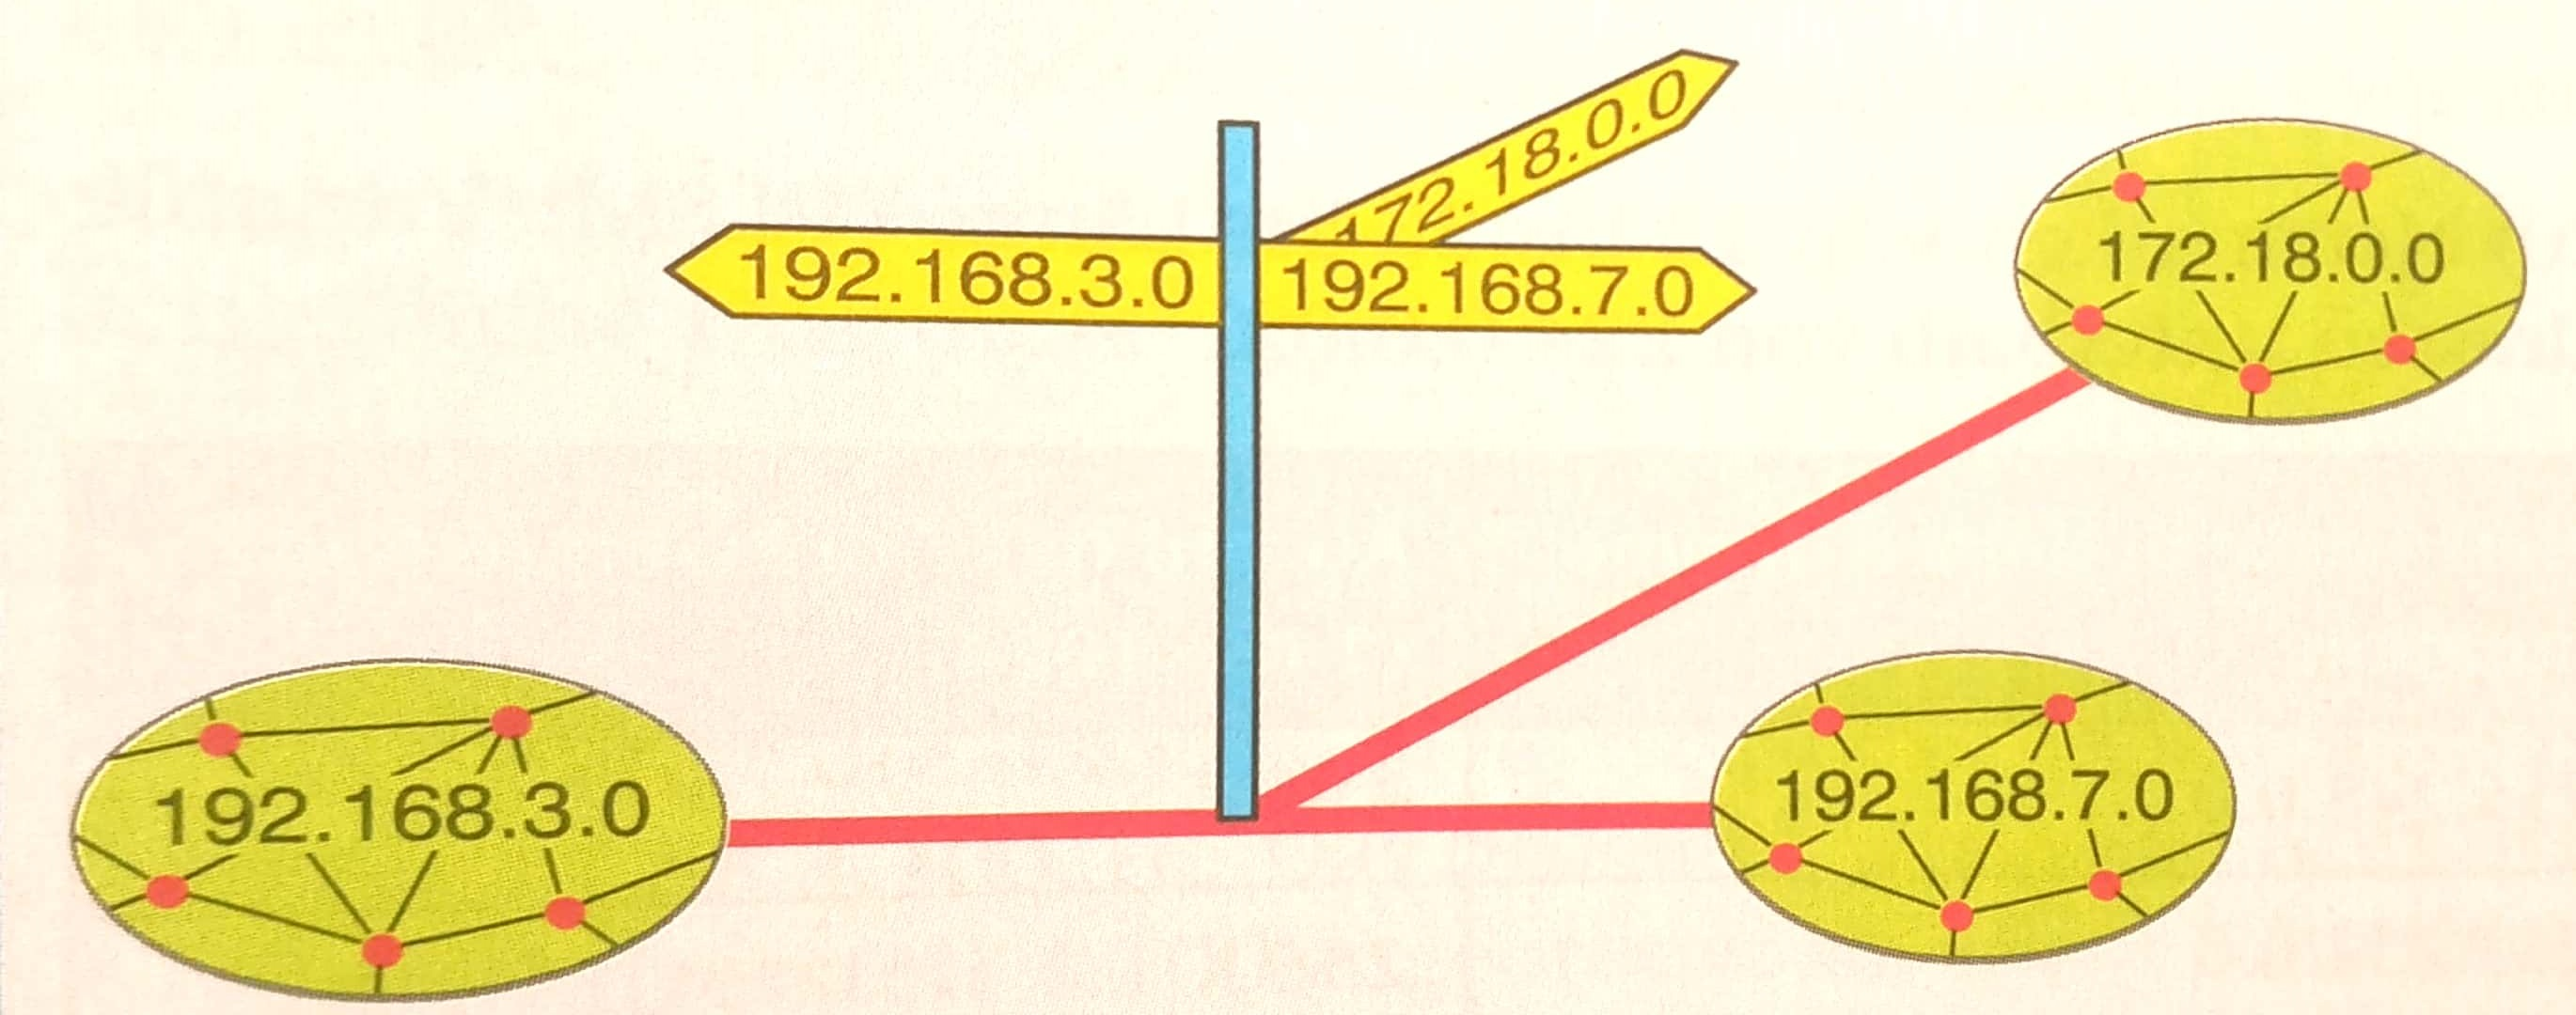
\includegraphics[width=\textwidth]{../99_Bilder/041_Skr_Sonder.jpg}
		\subsection{Bildung von Subnetzen}
		Es kann manchmal notwendig sein, innerhalb eines Netzes (z.B. 11.88.0.0/16) kleinere Subnetze zu bilden.\\
		Hierbei muss man zunächst folgende Frage klären:
		\begin{enumerate}
			\item Kenne ich die Anzahl der Subnetze?
			\item Kenne ich die Anzahl der Hosts pro Subnetz?
		\end{enumerate}
		Welche Frage wir mit \textit{\underline{ja}} beantworten bestimmt unser weiteres Vorgehen.
		\subsubsection{Kenne ich die Anzahl der Subnetze}
		Wir spielen den Prozess an oben genanntem Beispiel 11.88.0.0/16. Angenommen wir möchten 4 Subnetze bilden. Dann bestimmen wir die Anzahl der Bits, die wir benötigen, um 4 darzustellen - also \(2^x = 4\)\footnote{Ist die Anzahl der Subnetze keine Zweierpotenz, nehmen wir die nächst größere Zweierpotenz. Bei 12 Subnetzen, nutzen wir die 16.}. In unserem Fall sind das 2 Bit.\\
		Haben wir dies getan, erweitern wir also die bereits bekannte Netzmaske um zwei Bit. Die vier verschiedenen Status der zwei Bits markieren dann die Subnetze.\\
		\par\noindent
		\renewcommand{\arraystretch}{1.5}
		\begin{tabularx}{0.8\textwidth}{|L{0.12cm}|L{0.12cm}|L{0.12cm}|L{0.12cm}|L{0.12cm}|L{0.12cm}|L{0.12cm}|L{0.12cm}|L{0.12cm}|L{0.12cm}|L{0.12cm}|L{0.12cm}|L{0.12cm}|L{0.12cm}|L{0.12cm}|L{0.12cm}|L{0.12cm}|L{0.12cm}|L{0.12cm}|L{0.12cm}|L{0.12cm}|L{0.12cm}|L{0.12cm}|L{0.12cm}|L{0.12cm}|L{0.12cm}|L{0.12cm}|L{0.12cm}|L{0.12cm}|L{0.12cm}|L{0.12cm}|L{0.12cm}|}
			\cline{1-32}
			\rowcolor{blue!5} \multicolumn{8}{|c|}{\textbf{1. Byte}} & \multicolumn{8}{|c|}{\textbf{2. Byte}} & \multicolumn{8}{|c|}{\textbf{3. Byte}} & \multicolumn{8}{|c|}{\textbf{4. Byte}}\\
			\cline{1-32}
			0 & 0 & 0 & 0 & 1 & 0 & 1 & 1 &
			0 & 1 & 0 & 1 & 1 & 0 & 0 & 0 &
			\color{red}{0} & \color{red}{0}\normalcolor & X & X & X & X & X & X &
			X & X & X & X & X & X & X & X\\
			\cline{1-32}
			\multicolumn{16}{|c|}{Netzadressteil} &  \multicolumn{2}{c}{+2} & \multicolumn{14}{|c|}{Hostadressteil}\\
			\cline{1-32}
		\end{tabularx}\\
		\par\noindent
		\begin{tabbing}
			Netzadresse: ~~~~~~ \= 11.88.0.0/18\\
			Broadcastadresse: \> 11.88.63.255
		\end{tabbing}
		\par\noindent
		\renewcommand{\arraystretch}{1.5}
		\begin{tabularx}{0.8\textwidth}{|L{0.12cm}|L{0.12cm}|L{0.12cm}|L{0.12cm}|L{0.12cm}|L{0.12cm}|L{0.12cm}|L{0.12cm}|L{0.12cm}|L{0.12cm}|L{0.12cm}|L{0.12cm}|L{0.12cm}|L{0.12cm}|L{0.12cm}|L{0.12cm}|L{0.12cm}|L{0.12cm}|L{0.12cm}|L{0.12cm}|L{0.12cm}|L{0.12cm}|L{0.12cm}|L{0.12cm}|L{0.12cm}|L{0.12cm}|L{0.12cm}|L{0.12cm}|L{0.12cm}|L{0.12cm}|L{0.12cm}|L{0.12cm}|}
			\cline{1-32}
			\rowcolor{blue!5} \multicolumn{8}{|c|}{\textbf{1. Byte}} & \multicolumn{8}{|c|}{\textbf{2. Byte}} & \multicolumn{8}{|c|}{\textbf{3. Byte}} & \multicolumn{8}{|c|}{\textbf{4. Byte}}\\
			\cline{1-32}
			0 & 0 & 0 & 0 & 1 & 0 & 1 & 1 &
			0 & 1 & 0 & 1 & 1 & 0 & 0 & 0 &
			\color{red}{0} & \color{red}{1}\normalcolor & X & X & X & X & X & X &
			X & X & X & X & X & X & X & X\\
			\cline{1-32}
			\multicolumn{16}{|c|}{Netzadressteil} &  \multicolumn{2}{c}{+2} & \multicolumn{14}{|c|}{Hostadressteil}\\
			\cline{1-32}
		\end{tabularx}\\
		\par\noindent
		\begin{tabbing}
			Netzadresse: ~~~~~~ \= 11.88.64.0/18\\
			Broadcastadresse: \> 11.88.127.255
		\end{tabbing}
		\par\noindent
		\renewcommand{\arraystretch}{1.5}
		\begin{tabularx}{0.8\textwidth}{|L{0.12cm}|L{0.12cm}|L{0.12cm}|L{0.12cm}|L{0.12cm}|L{0.12cm}|L{0.12cm}|L{0.12cm}|L{0.12cm}|L{0.12cm}|L{0.12cm}|L{0.12cm}|L{0.12cm}|L{0.12cm}|L{0.12cm}|L{0.12cm}|L{0.12cm}|L{0.12cm}|L{0.12cm}|L{0.12cm}|L{0.12cm}|L{0.12cm}|L{0.12cm}|L{0.12cm}|L{0.12cm}|L{0.12cm}|L{0.12cm}|L{0.12cm}|L{0.12cm}|L{0.12cm}|L{0.12cm}|L{0.12cm}|}
			\cline{1-32}
			\rowcolor{blue!5} \multicolumn{8}{|c|}{\textbf{1. Byte}} & \multicolumn{8}{|c|}{\textbf{2. Byte}} & \multicolumn{8}{|c|}{\textbf{3. Byte}} & \multicolumn{8}{|c|}{\textbf{4. Byte}}\\
			\cline{1-32}
			0 & 0 & 0 & 0 & 1 & 0 & 1 & 1 &
			0 & 1 & 0 & 1 & 1 & 0 & 0 & 0 &
			\color{red}{1} & \color{red}{0}\normalcolor & X & X & X & X & X & X &
			X & X & X & X & X & X & X & X\\
			\cline{1-32}
			\multicolumn{16}{|c|}{Netzadressteil} &  \multicolumn{2}{c}{+2} & \multicolumn{14}{|c|}{Hostadressteil}\\
			\cline{1-32}
		\end{tabularx}\\
		\par\noindent
		\begin{tabbing}
			Netzadresse: ~~~~~~ \= 11.88.128.0/18\\
			Broadcastadresse: \> 11.88.191.255
		\end{tabbing}
		\par\noindent
		\renewcommand{\arraystretch}{1.5}
		\begin{tabularx}{0.8\textwidth}{|L{0.12cm}|L{0.12cm}|L{0.12cm}|L{0.12cm}|L{0.12cm}|L{0.12cm}|L{0.12cm}|L{0.12cm}|L{0.12cm}|L{0.12cm}|L{0.12cm}|L{0.12cm}|L{0.12cm}|L{0.12cm}|L{0.12cm}|L{0.12cm}|L{0.12cm}|L{0.12cm}|L{0.12cm}|L{0.12cm}|L{0.12cm}|L{0.12cm}|L{0.12cm}|L{0.12cm}|L{0.12cm}|L{0.12cm}|L{0.12cm}|L{0.12cm}|L{0.12cm}|L{0.12cm}|L{0.12cm}|L{0.12cm}|}
			\cline{1-32}
			\rowcolor{blue!5} \multicolumn{8}{|c|}{\textbf{1. Byte}} & \multicolumn{8}{|c|}{\textbf{2. Byte}} & \multicolumn{8}{|c|}{\textbf{3. Byte}} & \multicolumn{8}{|c|}{\textbf{4. Byte}}\\
			\cline{1-32}
			0 & 0 & 0 & 0 & 1 & 0 & 1 & 1 &
			0 & 1 & 0 & 1 & 1 & 0 & 0 & 0 &
			\color{red}{1} & \color{red}{1}\normalcolor & X & X & X & X & X & X &
			X & X & X & X & X & X & X & X\\
			\cline{1-32}
			\multicolumn{16}{|c|}{Netzadressteil} &  \multicolumn{2}{c}{+2} & \multicolumn{14}{|c|}{Hostadressteil}\\
			\cline{1-32}
		\end{tabularx}\\
		\par\noindent
		\begin{tabbing}
			Netzadresse: ~~~~~~ \= 11.88.192.0/18\\
			Broadcastadresse: \> 11.88.255.255
		\end{tabbing}
		Für den Hostadressteil verbleiben uns also 14 Bit. Das bedeutet jedes Subnetz besteht aus:
		\[\underbrace{1\ Netzadresse}_{11.88.X.0/18} + \underbrace{16382}_{2^{14}-2}\ Hostadressen + \underbrace{1\ Broadcastadresse}_{11.88.X.255} = 16384 = 2^14\]
		Eine Nachricht von außerhalb an einen Host wird immer noch an die Netzadresse \(11.88.0.0/16\) gesendet. Von dort wird sie an das richtige Subnetz weitergeleitet.
		\subsubsection{Kenne ich die Anzahl der Hosts pro Subnetz}
		Wissen wir hingegen, dass wir innerhalb des Netzes 11.88.0.0/16 Subnetze mit jeweils 4000 Hosts unterbringen, so gehen wir etwas anders vor.\\
		\par\noindent
		Zunächst bestimmen wir die Anzahl der Bits, die wir benötigen, um 4000 Hosts zu bedienen - also \(2^x \geq 4000\). Wir benötigen also \textbf{12 Bits} im \textbf{Hostadressteil}, so dass wir die geforderte Anzahl an Hosts unterbringen können.\\
		Von den 16 Bits des Hostadressteils reservieren wir also 12 für die geforderten Hosts. Die \textbf{übrigen 4 Bit} können wir nutzen, um \textbf{Subnetze zu bilden}. Wir können also \(2^4 = 16\) Subnetze bilden.\\
		\par\noindent
		\renewcommand{\arraystretch}{1.5}
		\begin{tabularx}{0.8\textwidth}{|L{0.12cm}|L{0.12cm}|L{0.12cm}|L{0.12cm}|L{0.12cm}|L{0.12cm}|L{0.12cm}|L{0.12cm}|L{0.12cm}|L{0.12cm}|L{0.12cm}|L{0.12cm}|L{0.12cm}|L{0.12cm}|L{0.12cm}|L{0.12cm}|L{0.12cm}|L{0.12cm}|L{0.12cm}|L{0.12cm}|L{0.12cm}|L{0.12cm}|L{0.12cm}|L{0.12cm}|L{0.12cm}|L{0.12cm}|L{0.12cm}|L{0.12cm}|L{0.12cm}|L{0.12cm}|L{0.12cm}|L{0.12cm}|}
			\cline{1-32}
			\rowcolor{blue!5} \multicolumn{8}{|c|}{\textbf{1. Byte}} & \multicolumn{8}{|c|}{\textbf{2. Byte}} & \multicolumn{8}{|c|}{\textbf{3. Byte}} & \multicolumn{8}{|c|}{\textbf{4. Byte}}\\
			\cline{1-32}
			0 & 0 & 0 & 0 & 1 & 0 & 1 & 1 &
			0 & 1 & 0 & 1 & 1 & 0 & 0 & 0 &
			\color{red}{?} & \color{red}{?} & \color{red}{?} & \color{red}{?}\normalcolor & X & X & X & X &
			X & X & X & X & X & X & X & X\\
			\cline{1-32}
			\multicolumn{16}{|c|}{Netzadressteil} &  \multicolumn{4}{c|}{+4} & \multicolumn{12}{c|}{Hostadressteil}\\
			\cline{1-32}
		\end{tabularx}\\
		\par\noindent
		Hier folgt dann wieder das gleiche Vorgehen, wie in 1.3.1 angedeutet. Wir gehen alle möglichen Belegungen der vier Bit durch und geben die Netz- wie auch die Broadcastadresse an.\\
		\par\noindent
		\begin{tabbing}
			Netzadressen: ~~~~~~ \= 11.88.0.0/20 ~~ \= 11.88.16.0/20 ~~ \= 11.88.32.0/20 ~~ \= 11.88.48.0/20\\
			Broadcastadresse: \> 11.88.15.255 \> 11.88.31.255 \> 11.88.47.255 \> 11.88.63.255\\
			\\
			Netzadressen: \> 11.88.64.0/20 \> 11.88.80.0/20 \> 11.88.96.0/20 \> 11.88.112.0/20\\
			Broadcastadresse: \> 11.88.79.255 \> 11.88.95.255 \> 11.88.111.255 \> 11.88.127.255\\
			\\
			Netzadressen: \> 11.88.128.0/20\> 11.88.144.0/20\> 11.88.160.0/20 \> 11.88.176.0/20\\
			Broadcastadressen: \> 11.88.143.255 \> 11.88.159.255 \> 11.88.175.255 \> 11.88.191.255\\
			\\
			Netzadressen: \> 11.88.192.0/20 \> 11.88.208.0/20 \> 11.88.224.0/20 \> 11.88.240.0/20\\
			Broadcastadressen: \> 11.88.207.255 \> 11.88.223.255 \> 11.88.239.255 \> 11.88.255.255
		\end{tabbing}
		\newpage
		\subsubsection*{Übersicht}
		Wie gehen Sie vor, um die Subnetze zu bestimmen:\\
		\par\noindent
		\begin{tabularx}{\textwidth}{|X|X|l|}
			\hline
			\rowcolor{gray!15}\textbf{Schritt} & \textbf{Rechnung} & \textbf{Beispiel}\\
			\hline
			Bits der Netzmaske angeben. Netzmaske binär aufschreiben & \multicolumn{2}{l|}{\footnotesize{Dezimal: 255.255.255.0 oder /24}}\\
			& \multicolumn{2}{l|}{\footnotesize{Binär: 1111 1111.1111 1111.1111 1111.0000 0000}}\\
			\hline
			\hline
			\textbf{Ich kenne die Anzahl der Subnetze} Berechne, wie viele Bits für das Subnetz notwendig sind & \footnotesize{Anzahl Subnetze =} \(2^x\) & \(4 = 2^2\)\\
			\hline
			Bestimmen, wie viele Bits noch für die Hostadresse bleiben. &\footnotesize{Hostbits ohne Subnetze - Bits für Subnetze} & \(6 = 8-2\)\\
			\hline
			Anzahl der bedienbaren Hosts in einem Subnetz & \footnotesize{Anzahl Hosts =} \(2^{Anzahl\ Hostbits\ pro\ Subnetz} - 2 \) & \(62 = 2^6 - 2\)\\
			\hline
			\hline
			\textbf{Ich kenne die Anzahl der Hosts pro Subnetz} Berechnen, wie viele Bits für die Hostanzahl benötigt werden. & \footnotesize{Anzahl Hosts =} \(2^x\) & \(64 = 2^6\)\\
			\hline
			Ausrechnen, wie viele Bits für die Subnetze übrig bleiben. & \footnotesize{Anzahl der Hostbits ohne Subnetze - Bits für Hostanzahl} & \(2 = 8 - 6\)\\
			\hline
			Anzahl der Subnetz bestimmen. & \footnotesize{Anzahl Subnetze =} \(2^{Anzahl\ Bits\ für\ Subnetze}\) & \(4 = 2^2\)\\
			\hline
			\hline
			Anzahl der Netzadress-Bits um die Anzahl der Bits für Subnetze erweitern. & \multicolumn{2}{l|}{\footnotesize{Binär: 1111 1111.1111 1111.1111 1111.1100 0000}}\\
			Neue Netzmaske binär schreiben. & \multicolumn{2}{l|}{\footnotesize{Dezimal: 255.255.255.192 oder /26}}\\
			\hline
		\end{tabularx}
	\end{worksheet}
\end{document}